
\documentclass[tikz]{standalone}
\usepackage{graphicx}
\usepackage{lmodern}
\usepackage{import}
\usepackage{amsmath, amssymb, amsfonts}
\usetikzlibrary{calc}
\newcommand{\R}{\mathcal{R}}
\newcommand{\conscvx}{\mathrm{cons}_\mathrm{cvx}}

\usetikzlibrary{arrows}

\begin{document}
	
	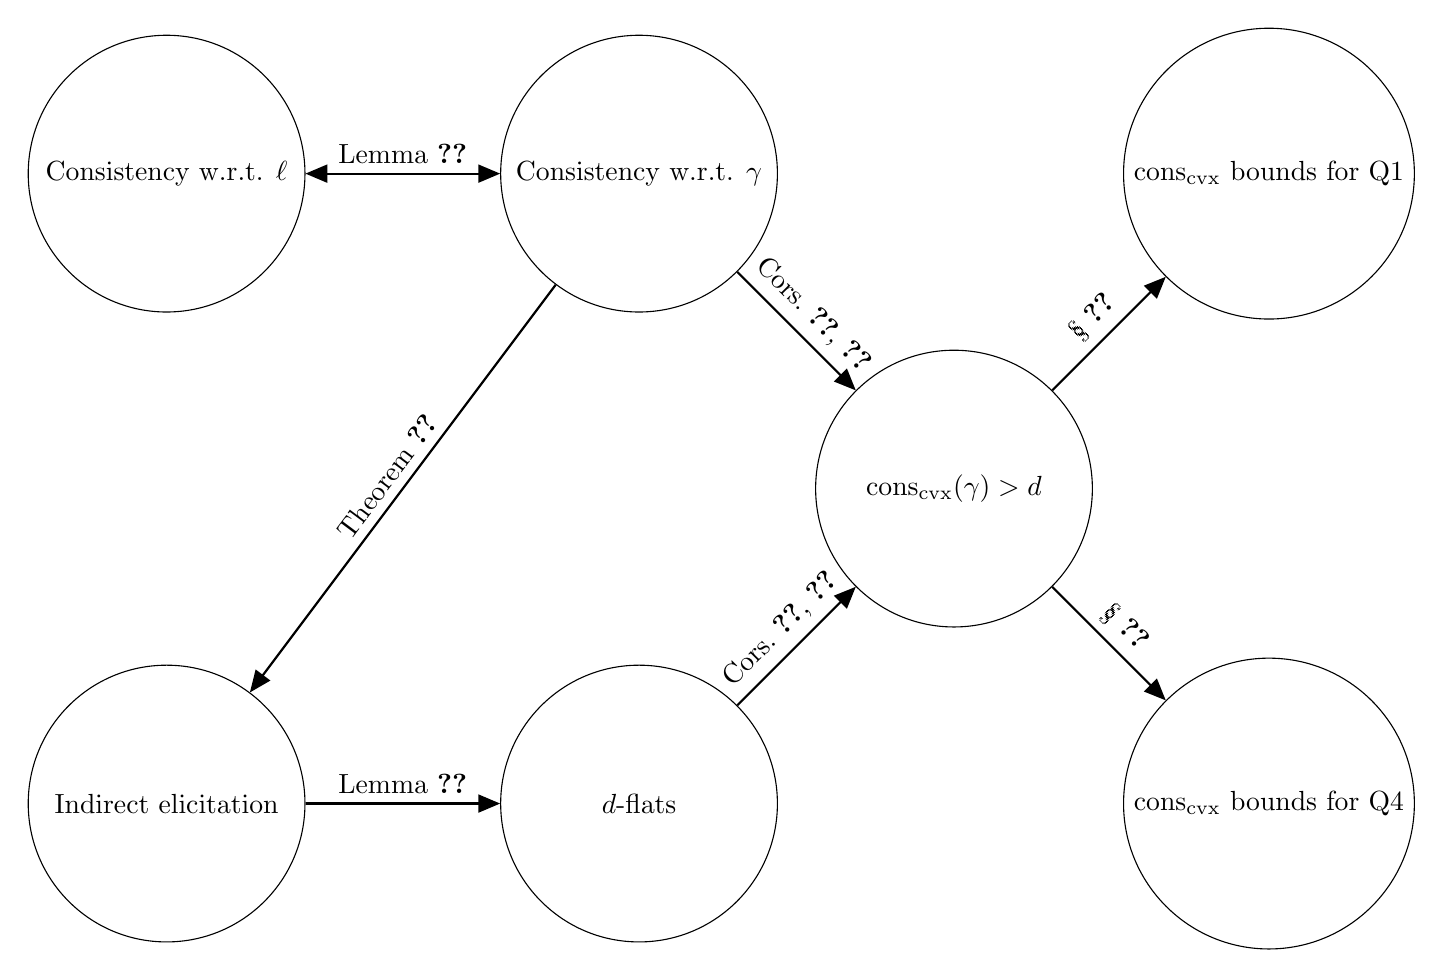
\begin{tikzpicture}
	
	\tikzset{vertex/.style = {shape=circle,draw,minimum size=10em}}
	\tikzset{edge/.style = {->,> = triangle 45, thick}}
	\tikzset{node/.style = {anchor=above, sloped}}
	
	% vertices
	\node[vertex] (consis-ell) at  (-2,4) {Consistency w.r.t. $\ell$};
	\node[vertex] (consis-gam) at  (4,4) {Consistency w.r.t. $\gamma$};
	\node[vertex] (indir-elic) at  (-2,-4) {Indirect elicitation};
	\node[vertex] (d-flats) at  (4,-4) {$d$-flats};
	\node[vertex] (conscvx-bd) at (8,0) {$\conscvx(\gamma) > d$};
	\node[vertex] (q1-bounds) at (12,4) {$\conscvx$ bounds for Q1};
	\node[vertex] (q4-bounds) at (12,-4) {$\conscvx$ bounds for Q4};
	
	%edges
	\draw[edge, <->] (consis-ell) to node[above]{Lemma~\ref{lem:consistent-loss-implies-prop}} (consis-gam);
	\draw[edge] (consis-gam) to node[above, sloped]{Theorem~\ref{thm:consistent-implies-indir-elic}} (indir-elic);
	\draw[edge] (indir-elic) to node[above, sloped]{Lemma~\ref{lem:convex-flats-inf-dim}} (d-flats);
	\draw[edge] (d-flats) to node[above, sloped]{Cors.~\ref{cor:Pcodim-flat-single-val-prop}, \ref{cor:Pcodim-flat-elic-relint-prop}} (conscvx-bd);
	\draw[edge] (consis-gam) to node[above, sloped]{Cors.~\ref{cor:Pcodim-flat-single-val-prop}, \ref{cor:Pcodim-flat-elic-relint-prop}} (conscvx-bd);
	\draw[edge] (conscvx-bd) to node[above, sloped]{\S~\ref{sec:finite-calib}} (q1-bounds);
	\draw[edge] (conscvx-bd) to node[above, sloped]{\S~\ref{sec:contin-consis}} (q4-bounds);
	
	\end{tikzpicture}
	
\end{document}